\documentclass{article}
\usepackage{PRIMEarxiv}
\usepackage[T1]{fontenc}
\usepackage[utf8]{inputenc}
\usepackage{xcolor}\usepackage{amsmath,amssymb,booktabs,tabularx,array,graphicx,microtype,hyperref}
\hypersetup{hidelinks,pdftitle={How Much Teammate Information Is Needed for Decentralized Fine Alignment of Two Robot Arms?},pdfauthor={Group 28, IIT Gandhinagar}}
\graphicspath{{media/}}
\fancyhead[L]{\small\itshape Decentralized Dual-Arm Fine Alignment}
\fancyhead[R]{\small Group 28 --- Multi-Agent Systems}
\setlength{\emergencystretch}{1.5em}
\setlength{\tabcolsep}{5pt}
\raggedbottom
% Generated from the verified episode analyses. Do not hand-edit numerical cells.
\newcommand{\LocalGap}{1.1}
\newcommand{\LocalCost}{2.356}
\newcommand{\OracleCost}{2.331}
\newcommand{\CapPayload}{152.4}
\newcommand{\BidPayload}{76.2}
\newcommand{\RgbAlignRange}{99.2--99.9}
\newcommand{\LearnedContactRange}{68.0--79.7}
\newcommand{\HalfInserted}{104}
\newcommand{\TruthInserted}{118}
\newcommand{\ContactDiff}{-21.9}
\newcommand{\ContactDiffCI}{-30.5, -14.1}
\newcommand{\BlockedInserted}{0}
\newcommand{\BlockedN}{64}
\newcommand{\BlockedReleased}{53}
\newcommand{\BlockedTried}{53}
\newcommand{\OpenReleased}{1}
\newcommand{\OpenTried}{11}
\newcommand{\LearnedPreFail}{151}
\newcommand{\LearnedDescentFail}{44}
\newcommand{\LearnedHoldFail}{1}
\newcommand{\LearnedPoseReject}{143}
\newcommand{\LearnedVisionReject}{8}
\newcommand{\AlignmentRows}{%
\multicolumn{5}{@{}l}{\textit{Deterministic allocation references (GT only)}} \\
S0 joint reference & 100.0 & 2.331 & -- & -- \\
S1 local model & 100.0 & 2.356 & -- & -- \\
Fixed half & 100.0 & 3.757 & -- & -- \\
\midrule
\multicolumn{5}{@{}l}{\textit{Learned policies: same frozen actor under GT and RGB}} \\
PPO S1 & 100.0 & 5.668 & 99.2 & 8.570 \\
PPO S2 & 100.0 & 4.645 & 99.6 & 5.908 \\
PPO S3 & 100.0 & 5.498 & 99.9 & 7.912 \\
PPO S4 & 100.0 & 5.309 & 99.5 & 7.402 \\
}
\newcommand{\FailureRows}{%
Learned RGB (six conditions) & 768 & 151 & 44 & 1 & 572 \\
Fixed-half RGB & 128 & 18 & 6 & 0 & 104 \\
S1 / ground truth & 128 & 0 & 10 & 0 & 118 \\
}

\newcommand{\RepositoryLink}{\url{https://github.com/single-spider/Decentralized-Alignment-of-Dual-Robot-Arm}}

\title{How Much Teammate Information Is Needed for\texorpdfstring{\\}{ }Decentralized Fine Alignment of Two Robot Arms?}
\author{Gaurav Srivastava \quad Aayush Bundel \quad Laxmidhar Swine \quad Roshin Gelasious\\[.4em]
Indian Institute of Technology Gandhinagar\\
Foundations of AI: Multiagent Systems \enspace $\cdot$ \enspace Group 28}


\setlength{\parskip}{4pt}
\setlength{\textfloatsep}{10pt plus 2pt minus 2pt}
\setlength{\intextsep}{9pt plus 2pt minus 2pt}
\newcommand{\takeaway}[1]{\par\noindent\textcolor{teal!65!black}{\textbf{#1}}\par}

\begin{document}
\maketitle
\thispagestyle{empty}
\begin{abstract}
Two robot arms can share a peg--fixture alignment correction, but their motion costs and knowledge of each other may differ. We compare local rules, capability messages, history-based prediction and pre-action bids with a full-information allocator. On 1,000 matched test cases for fit 0, a no-message rule succeeds on every case and costs only \LocalGap\% more in squared joint motion than the reference. Capability exchange closes that gap in this model; richer information offers no consistent improvement. We also train decentralized PPO actors and evaluate neural RGB sensing and dynamic contact insertion. RGB policies align on \RgbAlignRange\% of core starts, yet insert on only \LearnedContactRange\% across learned RGB open-hole conditions and do not outperform fixed-half RGB on insertion motion cost. Allocation, perception and contact execution therefore require separate evaluation.
\end{abstract}

\section{Introduction}
When a peg sits 4\,mm to the right of a hole, the peg arm can move left, the receiver arm can move right, or both can share the correction. Each choice can remove the same relative error, but the required joint movement depends on the robots' configurations. If both independently apply the full correction, they can overshoot; if both wait, the error remains.

\begin{figure}[!ht]
\centering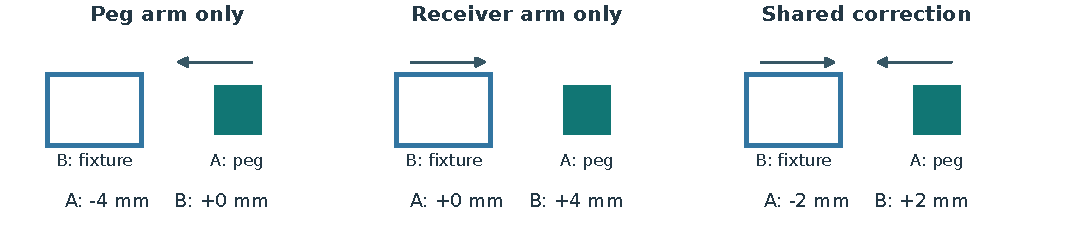
\includegraphics[width=\linewidth]{allocation-intuition.pdf}
\caption{Three allocations of a +4\,mm lateral error, shown schematically. Each gives the same relative correction; their joint-motion costs can differ. These illustrate total corrections, not single commands.}
\end{figure}

\textbf{Capability versus intent.} A teammate's kinematic cost describes which motions are cheaper, not which motion it will choose. A pre-action bid communicates intended effort, but its effect still depends on an agreed allocation convention.

\textbf{Research questions.} How closely can a no-message rule approach a joint allocator? What do capability messages, motion history and bids add? Does learned planar coordination remain effective with RGB sensing and physical contact in simulation?

\textbf{Study design.} We first hold sensing at ground truth to isolate allocation, then cross frozen learned actors with ground-truth and RGB sensing. A separate contact study tests whether visual alignment leads to completed insertion.

\clearpage
\subsection{Origin and scope}
Our work builds on the Seam Filling Network (SFN) of Xie et al.\ \cite{xie}, which segments the peg and seam to estimate lateral translation and yaw for visual feedback. The published physical-robot results belong to Xie et al., not this project. Before this course, Gaurav Srivastava implemented and studied the single-arm pipeline in simulation for his MTech thesis under Prof. Harish P M \cite{sfnsystem}. He discussed the proposed continuation with the course instructor, Prof. Manisha Padala, before submitting the project idea.

The thesis asks what correction one arm should execute; the course project asks how two arms should divide it. We reuse Panda and perception infrastructure, including the segmentation architecture and starting weights. New work comprises the shared two-arm environment, local information protocols, cost-aware comparisons, cooperative policy training, visual estimation for a moving receiver, and paired alignment/contact evaluation. Prior single-arm results provide background rather than evidence for the new controllers.

\begin{figure}[!ht]
\centering
\begin{minipage}[t]{.48\linewidth}\centering
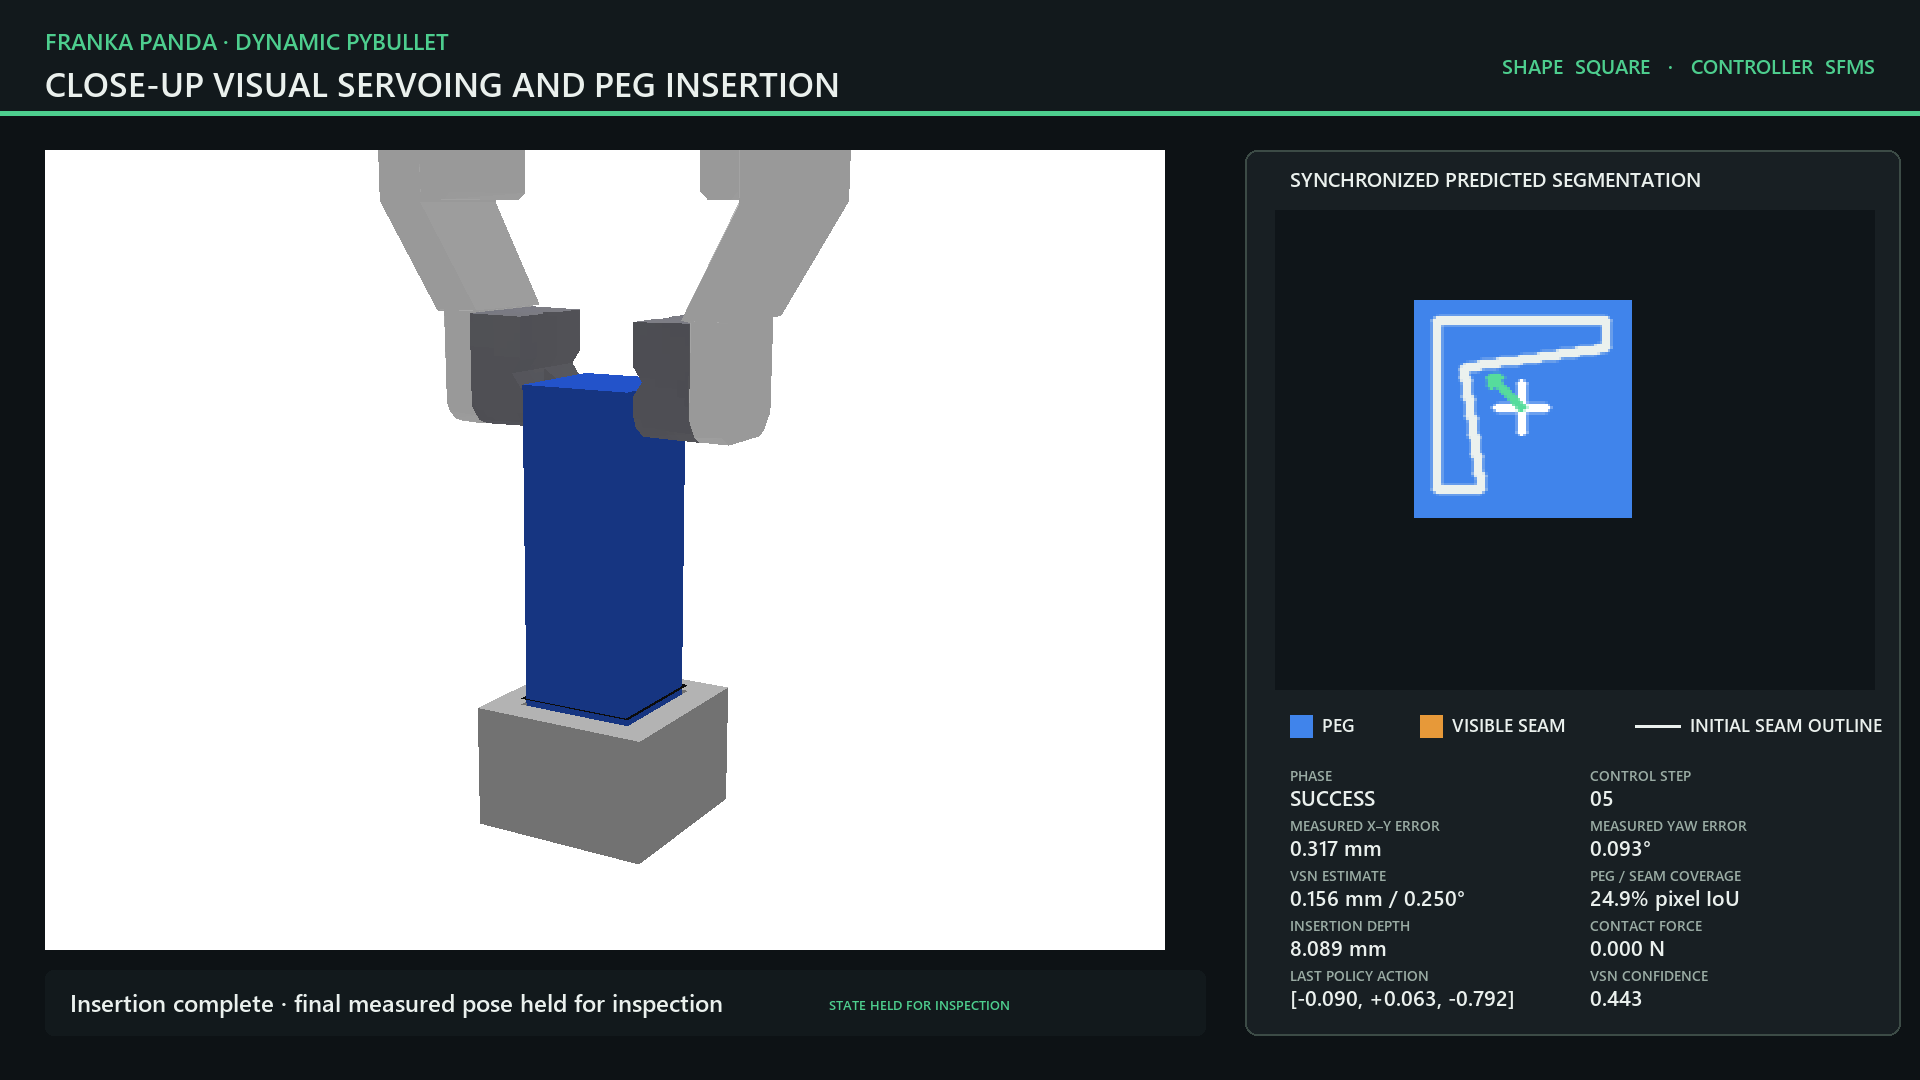
\includegraphics[width=\linewidth,height=1.42in,keepaspectratio]{single-arm.png}\\[-.1em]
\small (a) Prior MTech thesis: single-arm simulation
\end{minipage}\hfill
\begin{minipage}[t]{.48\linewidth}\centering
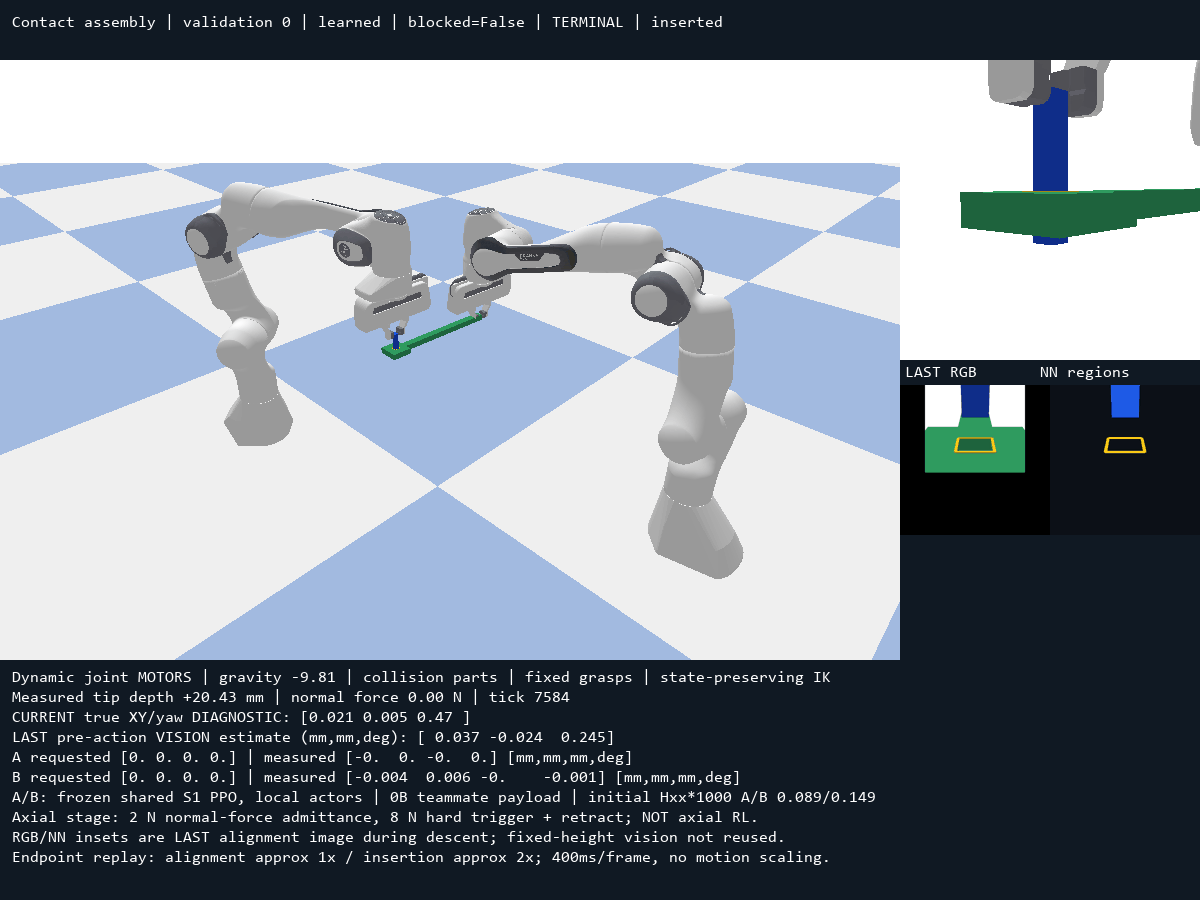
\includegraphics[width=\linewidth,height=1.42in,keepaspectratio]{dual-arm.png}\\[-.1em]
\small (b) Course study: both parts held and controlled
\end{minipage}
\caption{Prior single-arm SFN implementation (a) and an executed RGB-to-insertion replay from this course project (b). Neither image shows hardware. The full replay and frame sources are in the bundle.}
\label{fig:lineage}
\end{figure}


\section{Preliminaries}
Arm $A$ holds the peg and $B$ the fixture. The task error is peg minus fixture in a common world frame, with translations in metres and wrapped yaw in radians:
\begin{equation*}
 e=(\Delta x,\Delta y,\Delta\psi)^\top,
 \qquad e^+\simeq\operatorname{wrap}_\psi(e+a_A-a_B).
\end{equation*}
Each arm has seven joints $q_i$ and produces a signed held-reference increment $a_i$. Equal translations cancel in relative error. The update is a small-motion approximation; evaluation uses the executed held transforms measured in simulation.

\section{Problem formulation}
A centralized reference observes both configurations and allocates both corrections. Each local actor instead receives common sensed error, its own joints and cost, and only the extra information allowed by its regime. This is a cooperative partially observed decision problem \cite{bernstein}, with shared rewards and potentially different observations:
\begin{align*}
 s_t&=(e_t,q_{A,t},q_{B,t}), & a_{i,t}&\sim\pi_i(\cdot\mid h_{i,t}),\\
 J(\pi_A,\pi_B)&=\mathbb E\!\left[\sum_{t<T}\gamma^t r_t\right].
\end{align*}
Here $h_{i,t}$ is the available local history. The team maximizes $J$ subject to feasible per-arm actions and the information restrictions in Table~\ref{tab:protocol}. Alignment ends when both lateral errors are at most 1\,mm and yaw error at most $1^\circ$, or after 20 commands. Insertion is evaluated separately.

\clearpage
\section{Methodology}
\subsection{Measured world, allocation, and information}
One PyBullet instance manages both Panda robots. Policies observe the same pre-step state before either motion executes (Fig.~\ref{fig:workflow}). Alignment uses full-pose inverse kinematics (IK) and joint interpolation, without contact physics. Commands are limited to 2\,mm per lateral axis and 0.04\,rad yaw per arm; joint, IK and sampled collision constraints reject infeasible actions.

\begin{figure}[!ht]
\centering
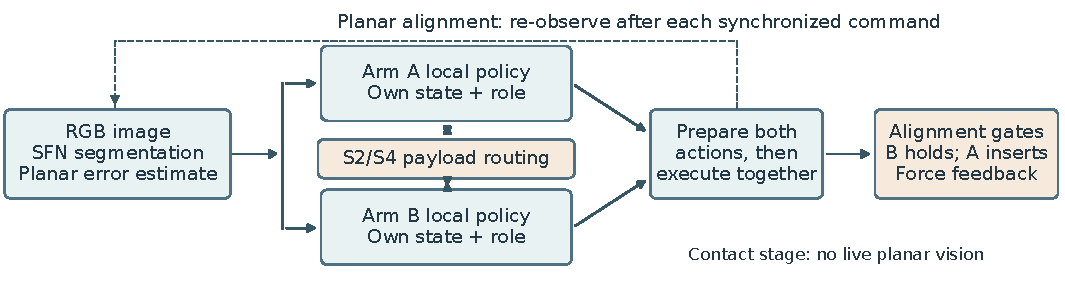
\includegraphics[width=\linewidth]{workflow.pdf}
\caption{Execution workflow. S1/S3 need no teammate messages; S2/S4 route permitted payloads before action selection. The GT comparison substitutes true planar error for the image estimate. Contact insertion begins only after alignment and pose checks.}
\label{fig:workflow}
\end{figure}


For normalized local increment $u_i$, finite differences at the held reference estimate the joint response $D_i$ while maintaining full-pose constraints:
\begin{equation*}
 \Delta q_i\approx D_i u_i,\qquad H_i=D_i^\top D_i,
 \qquad C=\sum_{t,i}\lVert q_{i,t+1}-q_{i,t}\rVert_2^2.
\end{equation*}
$H_i$ predicts squared joint displacement; $C$ measures executed motion. Because command subdivision can lower this sum, it is a motion metric rather than energy. We also record joint travel, command count, terminal error and payload.
\begin{table}[!ht]
\centering
\caption{Information available before execution; common sensing is excluded from payload.}
\begin{tabularx}{\linewidth}{@{}lXl@{}}
\toprule
Regime & Rule or additional information & Payload per command \\ \midrule
S0 & Joint cost allocation using both arms' capability. & Not decentralized \\[2pt]
S1 & Own cost plus a public cost prior: a shared model fitted before testing. & 0 bytes \\[2pt]
S2 & Other arm's symmetric $3\times3$ local cost matrix. & 48 bytes, one round \\[2pt]
S3 & Belief from past shared error changes and own executed motion. & 0 bytes \\[2pt]
S4 & Independent public local-model bids, routed before final actions. & 24 bytes, one round \\
\bottomrule
\end{tabularx}
\label{tab:protocol}
\end{table}


\textbf{Allocation convention.} One-arm-only and fixed-half controls divide the same correction. S0 searches a 125-point grid for the lowest predicted one-step cost, rather than a globally optimal trajectory:
\begin{align*}
 c&=\operatorname{clip}(e/s,-1,1),\quad s=(.002,.002,.04),
 & f&\in\{0,.25,.5,.75,1\}^3,\\
 u_A&=-f\odot c,\quad u_B=(1-f)\odot c,
 & f^*&\in\arg\min_f\bigl(u_A^\top H_Au_A+u_B^\top H_Bu_B\bigr).
\end{align*}
S1 replaces current teammate capability with a public prior fitted before testing. S2 exchanges cost matrices, letting both agents reconstruct S0's objective and agreed tie-break rule. Its match to S0 therefore relies on a shared allocation convention, even though execution is decentralized.

S3 combines a fitted prior with four past transitions in an expected-loss search. For A, past teammate motion is reconstructed as
\begin{equation*}
 \widehat a_B=a_A^{\rm exec}-(e^+-e),\qquad\text{with wrapped yaw.}
\end{equation*}
Noise affects this belief, and independently chosen shares need not sum to one correction. The fixed-belief control uses the same solver without history updates. S4 changes reconciliation as well as information through independent bids.

\textbf{Accounting and fits.} Float32 payload counts dropped transmissions but excludes headers and common sensing. Fitted models face the same held-out starts. Each development/model seed pair defines a \emph{fit}; \emph{fit 0} is the first, not a separate test set.

\clearpage
\subsection{Cooperative PPO and visual observations}
\takeaway{Training shares team information; execution retains local information limits.}
We use centralized training and decentralized execution \cite{ppo,mappo}. A shared, role-conditioned actor selects a fraction from $\{0,.25,.5,.75,1\}$ for each axis. Arm A acts opposite to the clipped sensed error and B in the same direction, each scaled by its own fraction. The geometric scaffold supplies direction, not the joint split: the actors can contribute unequally or over- and under-correct. Missing information slots are zero.

\begin{figure}[!ht]
\centering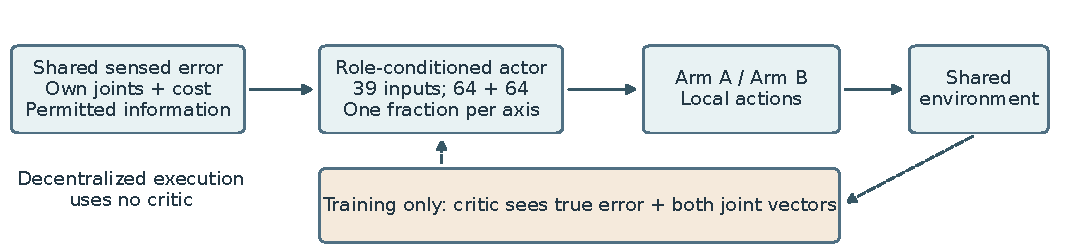
\includegraphics[width=\linewidth]{training-execution.pdf}
\caption{Shared actor architecture, evaluated separately for each arm. Permitted information depends on the regime. The critic and its privileged inputs are used only during training; both actors receive the same team advantage.}
\end{figure}

\textbf{Reward and optimization.} A 17-input critic observes true relative error and both joint vectors. With tolerance vector $\tau$, command motion $C_t$ and payload $B_t$, the base reward is
\begin{equation*}
 r_t^{\rm base}=-\lVert e^+/\tau\rVert_2^2-1000C_t-10^{-4}B_t-.01
       +10\,\mathbf 1_{\rm success}-10\,\mathbf 1_{\rm invalid}.
\end{equation*}
Training additionally subtracts 10,000 on invalid termination or timeout, then scales the reward by $.01$. This prevents early failure from becoming an inexpensive alternative to progress.

\begin{table}[!ht]\centering
\caption{Network and PPO settings. All 12 fits reach at least 10,000 environment steps.}
\begin{tabularx}{\linewidth}{@{}lXlX@{}}\toprule
Actor & 39 inputs; two 64-unit layers & Critic & 17 inputs \\
GAE $(\gamma,\lambda)$ & $(.99,.95)$ & PPO clip & 0.2 \\
Optimizer & Adam & Learning rate & $3\times10^{-4}$ \\
\bottomrule\end{tabularx}
\end{table}

Early and late candidates were ranked by held-out validation success, then cost and commands. Test evaluation uses the frozen selected actor. Validation favored probability-weighted mean fractions over modal decoding, which sometimes oscillated.

\textbf{Active RGB loop.} A calibrated camera follows the receiver through its grasp frame. A fine-tuned SFN segmenter predicts peg and seam regions from each pre-action image. Silhouette fitting and ring-plane rectification convert these regions to planar error. Color refinement stays within the neural proposals; invalid masks are rejected rather than replaced with true pose.

Simulator IDs label the 192 training and 24 validation RGB frames. Execution uses neither those IDs nor depth imaging, and true error is not an RGB actor input. Both actors receive the same image-derived estimate. Known part geometry and pre-insertion height are assumptions of the estimator.

\clearpage
\subsection{Dynamic contact insertion and fixture}
\takeaway{Insertion is a separate dynamic test, not a consequence of alignment success.}
The contact simulation includes gravity, joint-position motors and rigid collision bodies with mass. Rigid constraints represent grasps, so the study evaluates coordinated assembly rather than frictional grasp stability. A rigid offset handle keeps the receiver-arm attachment away from the axial approach while leaving the opening visible. The blocked control adds an obstruction below the same entrance.

\begin{table}[!ht]\centering
\caption{Fixture geometry and contact-controller thresholds. All validation is in simulation.}
\begin{tabularx}{\linewidth}{@{}lXlX@{}}\toprule
Square peg & 10\,mm & Square opening & 14\,mm \\
Fixture thickness & 14\,mm & Nominal descent & 0.5\,mm/command \\
Axial setpoint & 2\,N & Sampled stop trigger & 8\,N total normal force \\
Insertion depth & 20\,mm & Hold / depth recheck & 1\,s / 19.5\,mm \\
Stall threshold & $<0.05$\,mm/command & Retraction after & Three stalls \\
Retraction bound & 2\,mm & Shared physics clock & 240\,Hz \\
\bottomrule\end{tabularx}
\end{table}

\begin{figure}[!ht]
\centering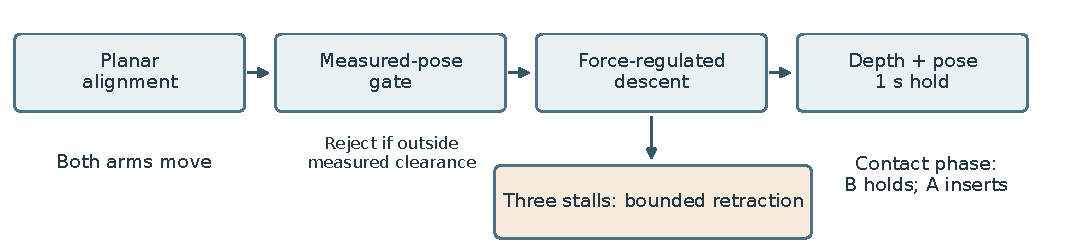
\includegraphics[width=\linewidth]{insertion-stages.pdf}
\caption{Contact execution after alignment. Measured geometry gates descent; force feedback regulates progress. Retraction is a bounded response to repeated stalls, not a guarantee of recovery.}
\end{figure}

\textbf{Gates and success.} After estimated alignment and a measured-pose check, B holds while A descends. Success requires 20\,mm measured tip depth, planar clearance and yaw checks, followed by a one-second simulated hold with a 19.5\,mm depth recheck. During changing height, control uses contact feedback and measured geometry rather than a stale planar vision estimate.

\textbf{Force-regulated progress.} At each physics tick, the command phase $z\in[0,1]$ updates as
\begin{align*}
 z^+&=\operatorname{clip}\!\left(z+
   \frac{\operatorname{clip}(1-F_{\rm axial}/(2\,\mathrm N),-.5,1)}{96},\,0,\,1\right),\\
 q_{\rm target}&=q_0+z(q_{\rm goal}-q_0).
\end{align*}
Joint motors track the interpolated target: forward progress slows near the setpoint and can briefly reverse above it. A stall is less than 0.05\,mm measured progress in a command. IK queries preserve the physics state, including contact and joint velocities.

\textbf{Stops and release.} An 8\,N sampled total-normal-force trigger and joint, penetration and grasp-drift guards stop unsafe progress. Three stalls can initiate an upward retraction of at most 2\,mm. Release requires more than 1\,mm tip backout, residual normal force below 1\,N and no new guard stop. The sampled trigger does not certify a peak-force cap, and rigid grasps do not establish hardware safety.

\clearpage
\section{Results}
\subsection{Teammate information versus motion and payload}
\textbf{Effective decentralized alignment required little communication in this model.} Both S0 and the S1 local-model controller aligned all 1,000 matched initial configurations for fit 0. Their mean squared joint-motion costs were \OracleCost{} and \LocalCost{} $\times10^{-3}$\,rad$^2$ per episode, a gap of only \LocalGap\%. Exchanging capability information (S2) removed that gap to displayed precision at \CapPayload{} bytes per episode. Explicit bids (S4) also approached the reference using approximately half that payload. Thus a shared allocation convention and suitable cost prior can substantially reduce the need for explicit teammate communication within the evaluated conditions.

\begin{figure}[!ht]
\centering
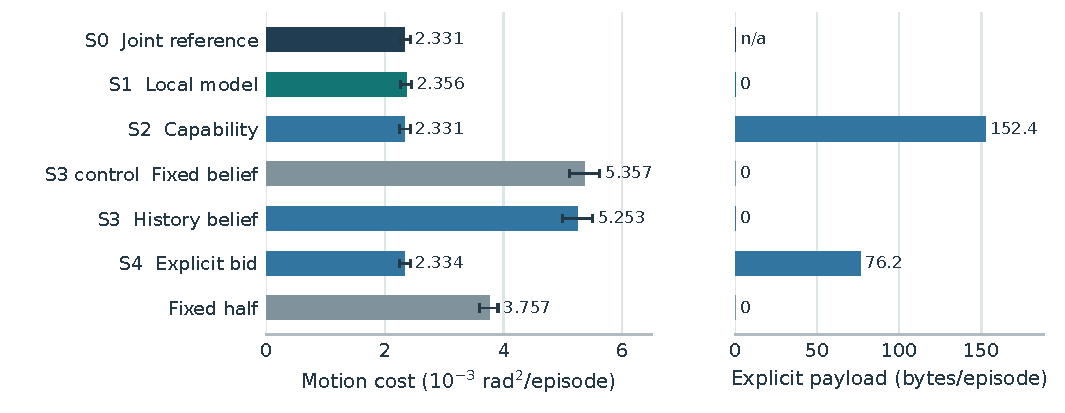
\includegraphics[width=\linewidth]{cost-payload.pdf}
\caption{Deterministic alignment for fit 0, 1,000 matched starts per method. Bars show means and episode bootstrap 95\% intervals for cost. Centralized information is not a comparable message payload. S3's fixed-belief control uses the same solver without history.}
\label{fig:payload}
\end{figure}

\subsection{What the experiments cover}

Table~\ref{tab:coverage} separates the three studies. Deterministic controls include one-arm, fixed-half and S0--S4 variants. The learned core crosses four regimes, three independent actor/data fits and two sensing modes, using 1,000 matched starts per entry. Each open-hole contact condition has 128 starts; blocked and stress conditions have 32 matched starts each. Corrected contact runs preserve Bullet state during IK; earlier diagnostic runs are excluded.

\begin{table}[!ht]\centering
\caption{Evaluation coverage. Contact is separate from alignment; its other trials comprise 64 blocked and 128 stress trials.}
\label{tab:coverage}
\begin{tabular}{@{}lrrr@{}}\toprule
Study & Core / open & Stress / other & Total \\\midrule
Deterministic alignment & 20,000 & 3,456 & 23,456 \\
Learned alignment & 24,000 & 1,280 & 25,280 \\
Dynamic contact & 1,024 & 192 & 1,216 \\
\bottomrule\end{tabular}
\end{table}

The principal alignment distribution uses feasible fine offsets within $\pm8$\,mm per lateral axis and $\pm0.18$\,rad in yaw (about $10.3^\circ$), not the proposal's wider target range. Separate camera checks cover feasible wider corners. The smaller stress panels include observation noise, delayed and dropped messages, unequal arm limits, tighter and looser tolerances, history length, and message precision. Neural RGB occlusion is tested separately. Changing history and comparing a fixed-belief control test predictor usefulness indirectly; we did not sweep externally prescribed prediction accuracy or repeat the full S0 comparison under every impairment. Paired intervals resample common starts; they do not substitute for independent fits or justify extrapolation beyond the tested range.

\clearpage
\subsection{Learned alignment and the cost of sensing}
Neural RGB achieved \RgbAlignRange\% alignment success across the 12 actor/regime fits. The same actors with ground-truth observations each aligned on 1,000/1,000 starts, typically with fewer commands and less squared motion. Table~\ref{tab:alignment} holds the actor fixed within each PPO row, isolating the sensing change. Under matched GT sensing, learned actors used fewer commands than fixed half, but all twelve used more squared motion. The learned actors achieve alignment, but the squared-motion comparison favors the deterministic fixed-half baseline. Comparisons between PPO regimes also change the fitted policy, not information alone.

\begin{table}[!ht]
\centering
\caption{Alignment on 1,000 matched test cases per entry for fit 0. Costs are in $10^{-3}$\,rad$^2$/episode; success is in percent. Compare GT and RGB within a PPO row for sensing, or GT columns across controller families. Dashes denote unevaluated RGB counterparts in this alignment benchmark.}
\begin{tabular}{@{}lrrrr@{}}
\toprule
& \multicolumn{2}{c}{Ground truth (GT)} & \multicolumn{2}{c}{Neural RGB} \\
\cmidrule(lr){2-3}\cmidrule(l){4-5}
Controller & Success & Cost & Success & Cost \\ \midrule
\AlignmentRows
\bottomrule
\end{tabular}
\label{tab:alignment}
\end{table}

\subsection{Transfer from visual alignment to insertion}
Across six learned RGB open-hole conditions, including the alternate S1 fits, insertion success ranged from \LearnedContactRange\%. Fixed-half RGB inserted on \HalfInserted/128 starts and S1 with true error on \TruthInserted/128. Holding the S1 actor fixed, RGB minus ground truth was \ContactDiff{} percentage points (paired 95\% interval [\ContactDiffCI]). A common failure was an estimated alignment that passed the vision gate but failed the measured yaw check before descent. There was no privileged correction fallback. All four first-fit learned RGB policies cost more than fixed-half RGB in the contact study, where controllers faced the same initial states; the paired cost intervals were above zero. The motion-cost comparison includes failures and measures endpoint joint displacement, not energy.

\begin{figure}[!ht]
\centering
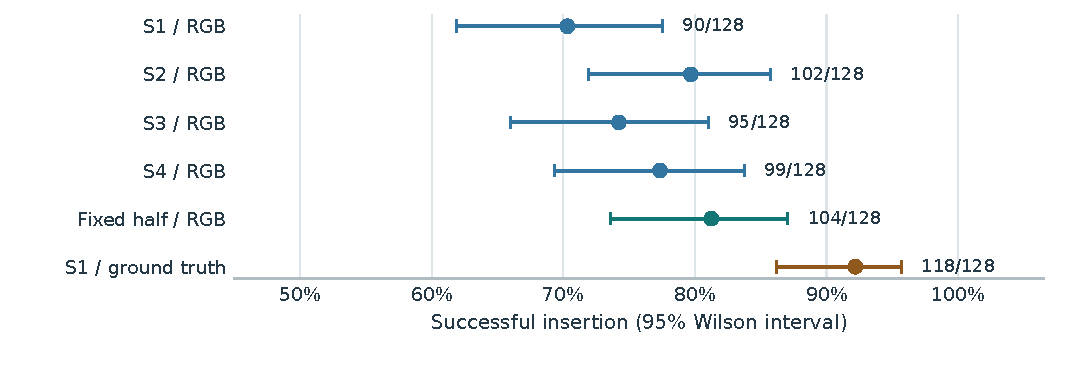
\includegraphics[width=\linewidth]{insertion-success.pdf}
\caption{Open-hole insertion on 128 matched starts per fit 0 condition. Points and Wilson intervals describe insertion, not the earlier alignment benchmark. Only the S1 RGB/ground-truth contrast holds the actor fixed.}
\label{fig:contact}
\end{figure}

\clearpage
\subsection{Where insertion failures occur}
Table~\ref{tab:failures} classifies every main open-hole trial by the stage at which it ended. Among the six learned RGB conditions, \LearnedPreFail{} trials failed before descent, \LearnedDescentFail{} during descent and \LearnedHoldFail{} during the hold. These are pooled counts across different fitted policies, not 768 independent model fits. Of the \LearnedPreFail{} pre-descent failures, \LearnedPoseReject{} were measured-pose rejections after visual alignment and \LearnedVisionReject{} failed the estimated-alignment gate. The separate alignment benchmark's high success therefore does not imply an equally high chance of completing dynamic assembly.

\begin{table}[!ht]
\centering
\caption{Main open-hole outcomes, excluding blocked and stress controls. Failure columns are mutually exclusive. A nonempty descent trace marks descent; a terminal-hold failure takes precedence. Counts, IDs and reasons are included in the bundle.}
\begin{tabular}{@{}lrrrrr@{}}
\toprule
Controller / sensing & N & Before descent & Descent & Hold & Inserted \\ \midrule
\FailureRows
\bottomrule
\end{tabular}
\label{tab:failures}
\end{table}

\subsection{Jam detection and retraction}
The blocked controls produced \BlockedInserted/\BlockedN{} false insertions and \BlockedReleased/\BlockedTried{} released retractions; the other starts were rejected before descent. Only \OpenReleased/\OpenTried{} attempted open-hole retractions released. Thus a controlled blockage verifies one jam response, not universal recovery. Figure~\ref{fig:traces} shows an actual paired validation replay: the open case reaches 20.43\,mm, while the blocked case stalls near the setpoint and retracts to 14.19\,mm with zero residual normal force.

\begin{figure}[!ht]
\centering
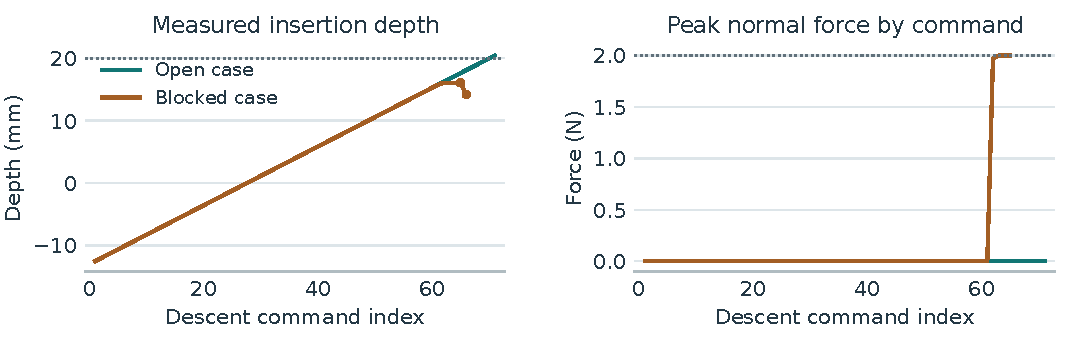
\includegraphics[width=\linewidth]{contact-traces.pdf}
\caption{Paired open/blocked replay with the same S1 RGB actor. Dotted lines mark the 20\,mm depth goal and 2\,N setpoint; the dashed final segment is retraction, not another descent. Selected traces illustrate behavior rather than population-level safety.}
\label{fig:traces}
\end{figure}

\section{Discussion and conclusion}
A shared convention and useful prior let local allocation approach the myopic joint reference without messaging. Capability removed a small cost gap; history and bids offered other speed/payload tradeoffs. These findings concern the evaluated allocation model; they do not identify a general minimum bandwidth, and the learned policies show no efficiency advantage over the tested baselines. Contact trials expose a separate transition from visual alignment to guarded insertion. Fixed grasps, one geometry family and sampled force checks limit hardware or safety conclusions. Future work should test whether learned axial corrections or earlier backoff improve insertion or recovery on matched starts at comparable force and travel limits.


\clearpage
\section{Reproduction}
\textbf{Repository:} \RepositoryLink

The README separates verification of saved results, a fresh RGB-to-contact replay, and fresh training/evaluation. The bundle contains held-out starts, source, configurations, selected and latest weights, optimizer and random-number-generator checkpoints, all 12 PPO fit logs, and vision-adaptation records. Raw episodes and the SHA-256 manifest support checking the results without retraining. Plots use recomputed study summaries and recorded replay telemetry; stopped contact diagnostics remain separately labeled.

\begin{table}[!ht]\centering
\caption{Seeds and held-out evaluation sets. Contact stress subsets use matched starts.}
\begin{tabularx}{\linewidth}{@{}lX@{}}\toprule
Allocation data / PPO model seeds & 311--313 / 401--403 \\
Validation & Seed 29; 24 starts \\
Alignment test & Seed 101; 1,000 starts \\
Contact benchmark & 128-start slice of the test manifest, unused for contact development \\
\bottomrule\end{tabularx}
\end{table}

\textbf{Selection and perception limits.} The late S1 candidate for fit 0 was originally ranked using a color-only RGB comparison. Its later matched-neural check is diagnostic; the frozen selection remains unchanged. Three actor fits share one vision checkpoint. The 24-image validation set supports selection only within this setup: vision was not independently retrained, and validation-size sensitivity was not studied. Between-actor variation therefore cannot establish robustness to perception training or model selection.

\section{Contributions}
The project was organized around complementary responsibilities covering system development, decentralized coordination, reinforcement learning, experimental evaluation, and research communication. All members contributed to project discussions, interpretation of findings, and review of the final report.

\begin{table}[!ht]\centering
\begin{tabularx}{\linewidth}{@{}p{.24\linewidth}X@{}}\toprule
Member & Responsibilities \\\midrule
Gaurav Srivastava & Formal modeling, simulator development and allocation baselines. \\
Aayush Bundel & Decentralized coordination, teammate prediction and message accounting. \\
Laxmidhar Swine & Cooperative reinforcement learning, training protocol and ablations. \\
Roshin Gelasious & Experimental design, analysis and robustness checks. \\
\bottomrule\end{tabularx}
\end{table}

\begin{thebibliography}{9}
\bibitem{xie} L. Xie, H. Yu, Y. Zhao, H. Zhang, Z. Zhou, M. Wang, Y. Wang, and R. Xiong. Learning to Fill the Seam by Vision: Sub-millimeter Peg-in-hole on Unseen Shapes in Real World. \emph{Proceedings of the IEEE International Conference on Robotics and Automation (ICRA)}, 2022. \href{https://arxiv.org/abs/2204.07776}{arXiv:2204.07776}.
\bibitem{sfnsystem} G. Srivastava. \emph{Submillimeter Accuracy Peg In Hole Insertion Using Seam Filling Network}. Single-arm research implementation and experimental study, IIT Gandhinagar. \url{https://single-spider.github.io/SFN/}.
\bibitem{bernstein} D. S. Bernstein, R. Givan, N. Immerman, and S. Zilberstein. The Complexity of Decentralized Control of Markov Decision Processes. \emph{Mathematics of Operations Research}, 27(4):819--840, 2002.
\bibitem{ppo} J. Schulman, F. Wolski, P. Dhariwal, A. Radford, and O. Klimov. Proximal Policy Optimization Algorithms. \emph{arXiv preprint}, 2017. \href{https://arxiv.org/abs/1707.06347}{arXiv:1707.06347}.
\bibitem{mappo} C. Yu et al. The Surprising Effectiveness of PPO in Cooperative Multi-Agent Games. \emph{Advances in Neural Information Processing Systems}, 35, 2022. \href{https://arxiv.org/abs/2103.01955}{arXiv:2103.01955}.
\end{thebibliography}
\end{document}
